% Für Bindekorrektur als optionales Argument "BCORfaktormitmaßeinheit", dann
% sieht auch Option "twoside" vernünftig aus
% Näheres zu "scrartcl" bzw. "scrreprt" und "scrbook" siehe KOMA-Skript Doku
\documentclass[12pt,a4paper,titlepage,headinclude,bibtotoc]{scrartcl}


%---- Allgemeine Layout Einstellungen ------------------------------------------

% Für Kopf und Fußzeilen, siehe auch KOMA-Skript Doku
\usepackage[komastyle]{scrpage2}
\pagestyle{scrheadings}
\automark[section]{chapter}
\setheadsepline{0.5pt}[\color{black}]

%keine Einrückung
\parindent0pt

%Einstellungen für Figuren- und Tabellenbeschriftungen
\setkomafont{captionlabel}{\sffamily\bfseries}
\setcapindent{0em}

\usepackage{caption}

%---- Weitere Pakete -----------------------------------------------------------
% Die Pakete sind alle in der TeX Live Distribution enthalten. Wichtige Adressen
% www.ctan.org, www.dante.de

% Sprachunterstützung
\usepackage[ngerman]{babel}

% Benutzung von Umlauten direkt im Text
% entweder "latin1" oder "utf8"
\usepackage[utf8]{inputenc}

% Pakete mit Mathesymbolen und zur Beseitigung von Schwächen der Mathe-Umgebung
\usepackage{latexsym,exscale,amssymb,amsmath}

% Weitere Symbole
\usepackage[nointegrals]{wasysym}
\usepackage{eurosym}

% Anderes Literaturverzeichnisformat
%\usepackage[square,sort&compress]{natbib}

% Für Farbe
\usepackage{color}

% Zur Graphikausgabe
%Beipiel: \includegraphics[width=\textwidth]{grafik.png}
\usepackage{graphicx}

% Text umfließt Graphiken und Tabellen
% Beispiel:
% \begin{wrapfigure}[Zeilenanzahl]{"l" oder "r"}{breite}
%   \centering
%   \includegraphics[width=...]{grafik}
%   \caption{Beschriftung} 
%   \label{fig:grafik}
% \end{wrapfigure}
\usepackage{wrapfig}

% Mehrere Abbildungen nebeneinander
% Beispiel:
% \begin{figure}[htb]
%   \centering
%   \subfigure[Beschriftung 1\label{fig:label1}]
%   {\includegraphics[width=0.49\textwidth]{grafik1}}
%   \hfill
%   \subfigure[Beschriftung 2\label{fig:label2}]
%   {\includegraphics[width=0.49\textwidth]{grafik2}}
%   \caption{Beschriftung allgemein}
%   \label{fig:label-gesamt}
% \end{figure}
\usepackage{subfigure}
\usepackage{adjustbox}

% Caption neben Abbildung
% Beispiel:
% \sidecaptionvpos{figure}{"c" oder "t" oder "b"}
% \begin{SCfigure}[rel. Breite (normalerweise = 1)][hbt]
%   \centering
%   \includegraphics[width=0.5\textwidth]{grafik.png}
%   \caption{Beschreibung}
%   \label{fig:}
% \end{SCfigure}
\usepackage{sidecap}

% Befehl für "Entspricht"-Zeichen
\newcommand{\corresponds}{\ensuremath{\mathrel{\widehat{=}}}}

%Für chemische Formeln (von www.dante.de)
%% Anpassung an LaTeX(2e) von Bernd Raichle
\makeatletter
\DeclareRobustCommand{\chemical}[1]{%
  {\(\m@th
   \edef\resetfontdimens{\noexpand\)%
       \fontdimen16\textfont2=\the\fontdimen16\textfont2
       \fontdimen17\textfont2=\the\fontdimen17\textfont2\relax}%
   \fontdimen16\textfont2=2.7pt \fontdimen17\textfont2=2.7pt
   \mathrm{#1}%
   \resetfontdimens}}
\makeatother

%Si Einheiten
\usepackage{siunitx}

%c++ Code einbinden
\usepackage{listings}
\lstset{numbers=left, numberstyle=\tiny, numbersep=5pt}

%Differential
\newcommand{\dif}{\ensuremath{\mathrm{d}}}

%Boxen,etc.
\usepackage{fancybox}
\usepackage{empheq}

%Fußnoten auf gleiche Seite
\interfootnotelinepenalty=1000

%Dateien aus Unterverzeichnissen
\usepackage{import}

%Bibliography \bibliography{literatur} und \cite{gerthsen}
%\usepackage{cite}
\usepackage{babelbib}
\selectbiblanguage{ngerman}

\begin{document}

\begin{titlepage}
\centering
\textsc{\Large Anfängerpraktikum der Fakultät für
  Physik,\\[1.5ex] Universität Göttingen}

\vspace*{4.2cm}

\rule{\textwidth}{1pt}\\[0.5cm]
{\huge \bfseries
  Messung von großen Widerständen\\[1.5ex]
  Protokoll:}\\[0.5cm]
\rule{\textwidth}{1pt}

\vspace*{3.0cm}

\begin{Large}
\begin{tabular}{ll}
Praktikant:
 	&  Felix Kurtz\\
 	&  Michael Lohmann\\

E-Mail: 
	&  felix.kurtz@stud.uni-goettingen.de\\
	& m.lohmann@stud.uni-goettingen.de\\

 Betreuer: & Björn Klaas\\
 Versuchsdatum: &  03.09.2014\\
\end{tabular}
\end{Large}

\vspace*{0.8cm}

\begin{Large}
\fbox{
  \begin{minipage}[t][2.5cm][t]{6cm} 
    Testat:
  \end{minipage}
}
\end{Large}

\end{titlepage}

\tableofcontents

\newpage

\section{Einleitung}
\label{sec:einleitung}
Um einen Widerstand zu messen, nutzt man meistens das Ohmsche Gesetz.
Ist der Widerstand jedoch hochohmig, stößt dieses Verfahren an seine Grenzen.
Man arbeitet mit hohen Spannungen und kleinen Strömen.
Außerdem sind die Innenwiderstände der Messgeräte ein großer Störfaktor.
Deshalb werden wir in diesem Versuch lernen, wie man das besser machen kann. 

\section{Theorie}
\label{sec:theorie}
\subsection{Messung mittels einem Kondensator}

\begin{align}
	Q(t)=Q_0 \exp \left(-\frac{t}{RC}\right)
\end{align}
Kennt man die Kapazität $C$ und die Ladung, die sich auf dem Kondensator befindet, zu zwei verschiedenen Zeitpunkten $t_1$ und $t_2$, kann man also den Widerstand $R$ berechnen, über den der Strom abfließt:
\begin{align}
	R=-\frac{t_2-t_1}{C\cdot\ln\frac{Q(t_2)}{Q(t_1)}}
\end{align}
Der hier verwendete Kondenstor hat einen Plattenradius $r=0.1~\si{\meter}$, einen Plattenabstand $d=0.005~\si{\meter}$ und eine Plattenzahl $n=65$.
Für die Berechnung der Kapazität müssen also Randeffekte betrachtet werden.
Dabei wird diese Formel verwendet:
\begin{align}	
	C_n=(n-1)\varepsilon_0\varepsilon_r\left[\frac{\pi r^2}{d}+r\left(\ln\frac{16\pi r}{d}-1\right)\right]
\end{align}
%ergibt sich eine Kapazität $C=3.896~\si{\nano\farad}$.

\subsection{Analoger Stromintegrator}
Nach der \textit{Kirchhoffschen Knotenregel} bei S gilt $I_R+I_C=0$.
Mit den folgenden Beziehungen der Ströme $I_R=U_E/R$ und $I_C=\dot{Q}_C=C\dot{U}_A$ erhält man:
\begin{align}
	U_A=-\frac{1}{RC}\int \limits_{t_0}^t U_E \,\dif t
\end{align}

\subsection{RLC-Schwingkreis}
\begin{align}
	\ddot{Q}+2\beta\dot{Q}+\omega_0^2 Q=0
\end{align}
\begin{align*}
	\beta=\frac{R_L}{2L} \quad , \quad 
	\omega_0=\sqrt{\frac{1}{LC}} \quad , \quad
	\omega=\sqrt{\omega_0^2-\beta^2}
\end{align*}
Mit dem Logarithmischen Dekrement $\Lambda=\beta T$ ergibt sich für die Induktivität der Spule
\begin{align}
	L=\frac{1}{C\omega_0^2}=\frac{1}{C(\omega^2+\beta^2)}=\frac{1}{C}\frac{T^2}{4\pi^2+\Lambda^2}
\end{align}
\begin{align}
	L=\mu_0 \cdot A \cdot \left(\frac{n}{l}\right)^2
\end{align}

\section{Durchführung}
\label{sec:durchfuehrung}

\section{Auswertung}
\label{sec:auswertung}
\subsection{Kalibration des Ladungsmessgerätes}
\begin{figure}
 \centering
 % GNUPLOT: LaTeX picture with Postscript
\begingroup
  \makeatletter
  \providecommand\color[2][]{%
    \GenericError{(gnuplot) \space\space\space\@spaces}{%
      Package color not loaded in conjunction with
      terminal option `colourtext'%
    }{See the gnuplot documentation for explanation.%
    }{Either use 'blacktext' in gnuplot or load the package
      color.sty in LaTeX.}%
    \renewcommand\color[2][]{}%
  }%
  \providecommand\includegraphics[2][]{%
    \GenericError{(gnuplot) \space\space\space\@spaces}{%
      Package graphicx or graphics not loaded%
    }{See the gnuplot documentation for explanation.%
    }{The gnuplot epslatex terminal needs graphicx.sty or graphics.sty.}%
    \renewcommand\includegraphics[2][]{}%
  }%
  \providecommand\rotatebox[2]{#2}%
  \@ifundefined{ifGPcolor}{%
    \newif\ifGPcolor
    \GPcolortrue
  }{}%
  \@ifundefined{ifGPblacktext}{%
    \newif\ifGPblacktext
    \GPblacktexttrue
  }{}%
  % define a \g@addto@macro without @ in the name:
  \let\gplgaddtomacro\g@addto@macro
  % define empty templates for all commands taking text:
  \gdef\gplbacktext{}%
  \gdef\gplfronttext{}%
  \makeatother
  \ifGPblacktext
    % no textcolor at all
    \def\colorrgb#1{}%
    \def\colorgray#1{}%
  \else
    % gray or color?
    \ifGPcolor
      \def\colorrgb#1{\color[rgb]{#1}}%
      \def\colorgray#1{\color[gray]{#1}}%
      \expandafter\def\csname LTw\endcsname{\color{white}}%
      \expandafter\def\csname LTb\endcsname{\color{black}}%
      \expandafter\def\csname LTa\endcsname{\color{black}}%
      \expandafter\def\csname LT0\endcsname{\color[rgb]{1,0,0}}%
      \expandafter\def\csname LT1\endcsname{\color[rgb]{0,1,0}}%
      \expandafter\def\csname LT2\endcsname{\color[rgb]{0,0,1}}%
      \expandafter\def\csname LT3\endcsname{\color[rgb]{1,0,1}}%
      \expandafter\def\csname LT4\endcsname{\color[rgb]{0,1,1}}%
      \expandafter\def\csname LT5\endcsname{\color[rgb]{1,1,0}}%
      \expandafter\def\csname LT6\endcsname{\color[rgb]{0,0,0}}%
      \expandafter\def\csname LT7\endcsname{\color[rgb]{1,0.3,0}}%
      \expandafter\def\csname LT8\endcsname{\color[rgb]{0.5,0.5,0.5}}%
    \else
      % gray
      \def\colorrgb#1{\color{black}}%
      \def\colorgray#1{\color[gray]{#1}}%
      \expandafter\def\csname LTw\endcsname{\color{white}}%
      \expandafter\def\csname LTb\endcsname{\color{black}}%
      \expandafter\def\csname LTa\endcsname{\color{black}}%
      \expandafter\def\csname LT0\endcsname{\color{black}}%
      \expandafter\def\csname LT1\endcsname{\color{black}}%
      \expandafter\def\csname LT2\endcsname{\color{black}}%
      \expandafter\def\csname LT3\endcsname{\color{black}}%
      \expandafter\def\csname LT4\endcsname{\color{black}}%
      \expandafter\def\csname LT5\endcsname{\color{black}}%
      \expandafter\def\csname LT6\endcsname{\color{black}}%
      \expandafter\def\csname LT7\endcsname{\color{black}}%
      \expandafter\def\csname LT8\endcsname{\color{black}}%
    \fi
  \fi
  \setlength{\unitlength}{0.0500bp}%
  \begin{picture}(7200.00,5040.00)%
    \gplgaddtomacro\gplbacktext{%
      \csname LTb\endcsname%
      \put(1254,704){\makebox(0,0)[r]{\strut{} 100}}%
      \put(1254,1213){\makebox(0,0)[r]{\strut{} 200}}%
      \put(1254,1722){\makebox(0,0)[r]{\strut{} 300}}%
      \put(1254,2231){\makebox(0,0)[r]{\strut{} 400}}%
      \put(1254,2740){\makebox(0,0)[r]{\strut{} 500}}%
      \put(1254,3249){\makebox(0,0)[r]{\strut{} 600}}%
      \put(1254,3758){\makebox(0,0)[r]{\strut{} 700}}%
      \put(1254,4267){\makebox(0,0)[r]{\strut{} 800}}%
      \put(1254,4776){\makebox(0,0)[r]{\strut{} 900}}%
      \put(1386,484){\makebox(0,0){\strut{} 100}}%
      \put(2005,484){\makebox(0,0){\strut{} 200}}%
      \put(2624,484){\makebox(0,0){\strut{} 300}}%
      \put(3243,484){\makebox(0,0){\strut{} 400}}%
      \put(3862,484){\makebox(0,0){\strut{} 500}}%
      \put(4482,484){\makebox(0,0){\strut{} 600}}%
      \put(5101,484){\makebox(0,0){\strut{} 700}}%
      \put(5720,484){\makebox(0,0){\strut{} 800}}%
      \put(6339,484){\makebox(0,0){\strut{} 900}}%
      \put(6958,484){\makebox(0,0){\strut{} 1000}}%
      \put(484,2740){\rotatebox{90}{\makebox(0,0){\strut{}Skalen-Teile}}}%
      \put(4172,154){\makebox(0,0){\strut{}Ladung [$\mu$C]}}%
    }%
    \gplgaddtomacro\gplfronttext{%
      \csname LTb\endcsname%
      \put(3762,4603){\makebox(0,0)[r]{\strut{}Messwerte}}%
      \csname LTb\endcsname%
      \put(3762,4383){\makebox(0,0)[r]{\strut{}Regressionsgerade}}%
    }%
    \gplbacktext
    \put(0,0){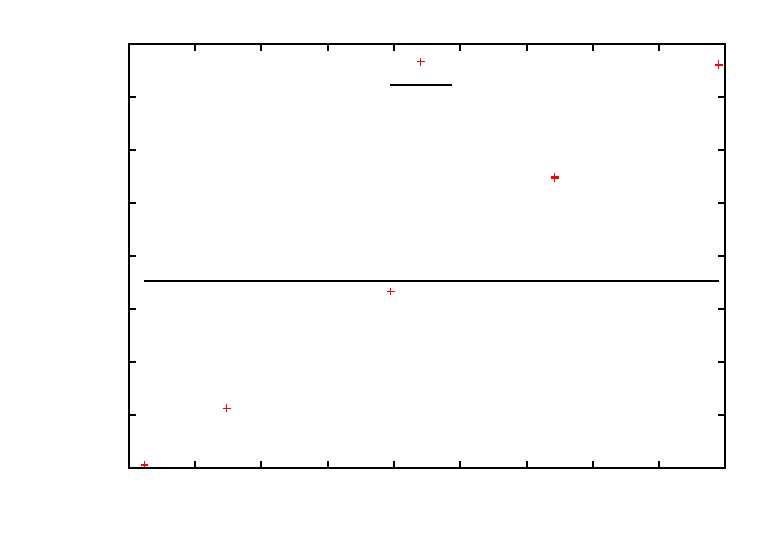
\includegraphics{Kalibration}}%
    \gplfronttext
  \end{picture}%
\endgroup

 \caption{Skalenteile des Messgeräts in Abhängigkeit der geflossenen Ladung}
 \label{fig:Kalibration}
\end{figure}

$$m=0.8729 \pm 0.0017 ~\text{Skt.}/\si{\micro\coulomb}$$

\subsection{Berechnung von $\varepsilon_0$ und Widerständen}

\begin{empheq}[box=\shadowbox*]{align}
	\varepsilon_0= \left(9.19 \pm 0.07\right)\cdot 10^{-12}\,\si[per-mode=fraction]{\ampere\second\per\volt\per\meter}
\end{empheq}
\subsection{Schwingkreise}

\section{Diskussion}
\label{sec:diskussion}

\section{Anhang}

\end{document}
